



\begin{figure*}
  \jsubfig{
\includegraphics[height=1.6cm]{figures/results/white_2.pdf}}{\begin{flushleft}\vspace{-6pt} \small{ Ours \footnotesize  (PViC+) \newline \vspace{-4pt}  \newline PViC \newline \vspace{-17pt} \newline \newline GT}
  \end{flushleft}} 
  \hfill
  \jsubfig{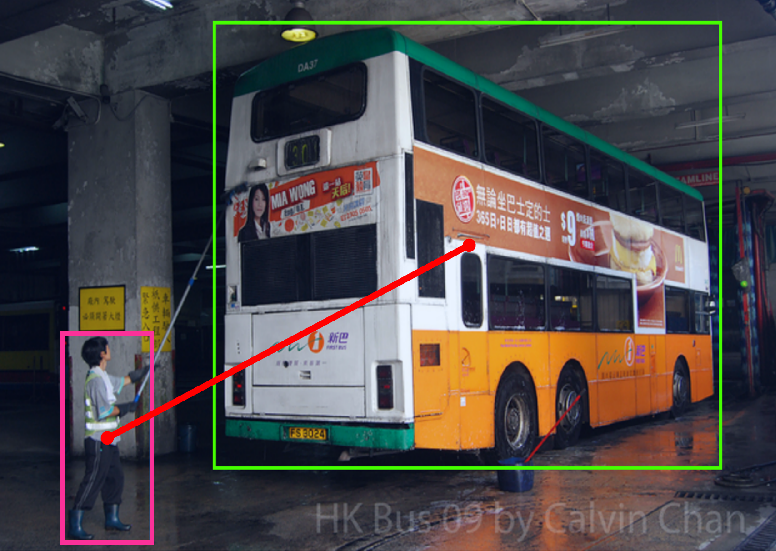
\includegraphics[height=3.6cm]{figures/results/hoi_washing.pdf}}{\vspace{-5pt}\begin{flushleft} \small \textcolor{red}{wash}
\\ \vspace{5pt}\textcolor{red}{-}  \\ \vspace{5pt} \textcolor{red}{washing a bus}  \\ %
  \end{flushleft}}
          \hfill
  \jsubfig{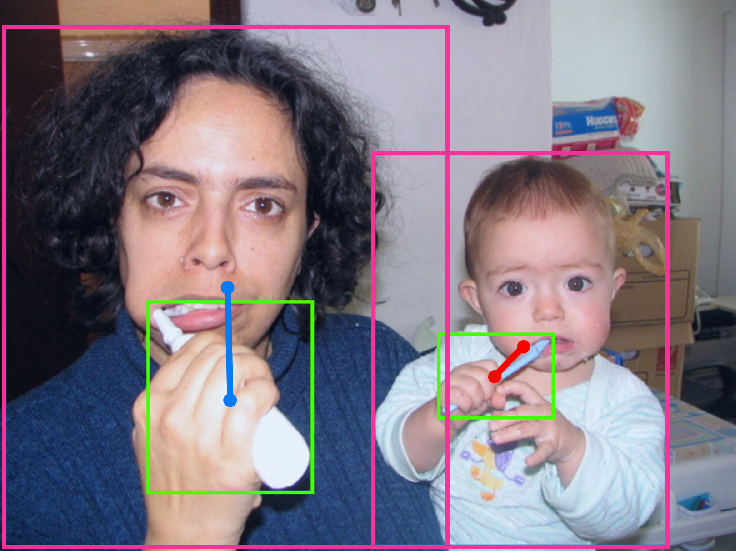
\includegraphics[height=3.6cm]{figures/results/hoi_brushing.pdf}}{\vspace{-5pt}\begin{flushleft} \small   \textcolor{blue}{ brush with, hold;} \textcolor{red}{brush with, hold} \\ \vspace{5pt}\textcolor{blue}{hold; }\textcolor{red}{ hold}  \\ \vspace{5pt}\textcolor{blue}{brushing with a toothbrush, holding
  \\a toothbrush;}  \textcolor{red}{brushing with a toothbrush, holding a toothbrush} \end{flushleft}}
          \hfill
  \jsubfig{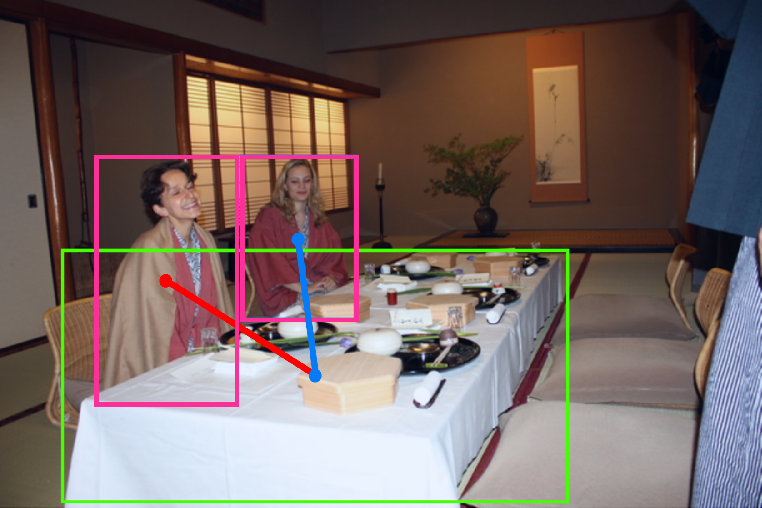
\includegraphics[height=3.6cm]{figures/results/hoi_siting.pdf}}{\vspace{-5pt}\begin{flushleft} \small{ \textcolor{blue}{sit at, eat at;} \textcolor{red}{sit at, eat at} \\ \vspace{5pt}  \textcolor{blue}{sit at;} \textcolor{red}{sit at}  \\\vspace{5pt}\textcolor{blue}{sitting at a table, eating at a table;} \textcolor{red}{sitting at a table, eating at a table} } \end{flushleft}}
          \hfill
  \caption{\textbf{HOI qualitative Comparison.} Example predictions of our \attentionmethod   (first row) and PViC~\cite{zhang2023pvic} (second row) on the HICO-DET~\cite{chao2015hico} test set.
    Predicted human and object bounding boxes are shown in \textcolor{Magenta}{pink} and \textcolor{ForestGreen}{green} respectively, and predicted interactions as a \textcolor{red}{red} and \textcolor{blue}{blue} lines, based on the description's interaction verbs colors.
    }
    \label{fig:hoi_results}
    \end{figure*}
